\section*{Результаты измерений}

Установим кювету с кристаллом на расстоянии $L = 80,0 \pm 0,5 \cm$. Осветим кристалл лазером через матовую пластину, получим на экране интерференционную картину. Лазерный свет поляризован в вертикальной плоскости.

\begin{figure}[H]
	\centering
	\begin{minipage}[b]{0.4\textwidth}
		\centering
		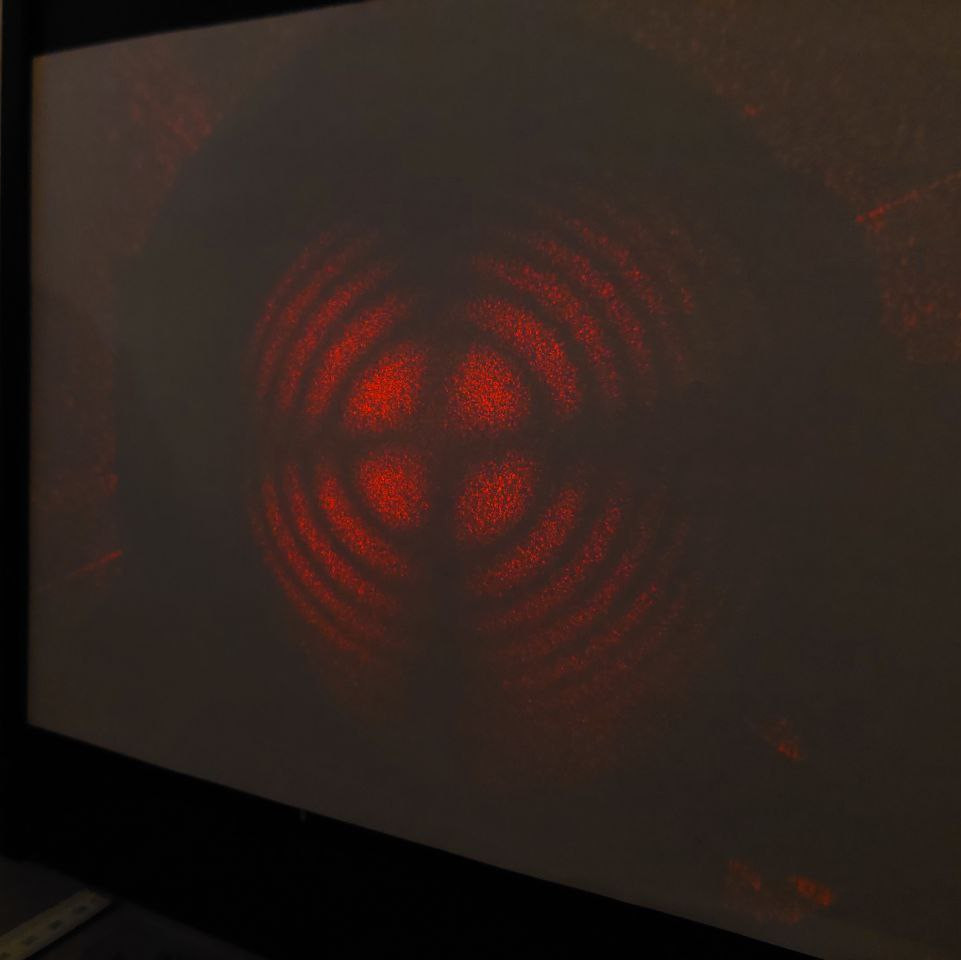
\includegraphics[width=\textwidth]{../Изображения/dark.jpg}
		\caption{Разрешённое направление анализатора горизонтально.}
	\end{minipage}
	\hfill
	\begin{minipage}[b]{0.4\textwidth}
		\centering
		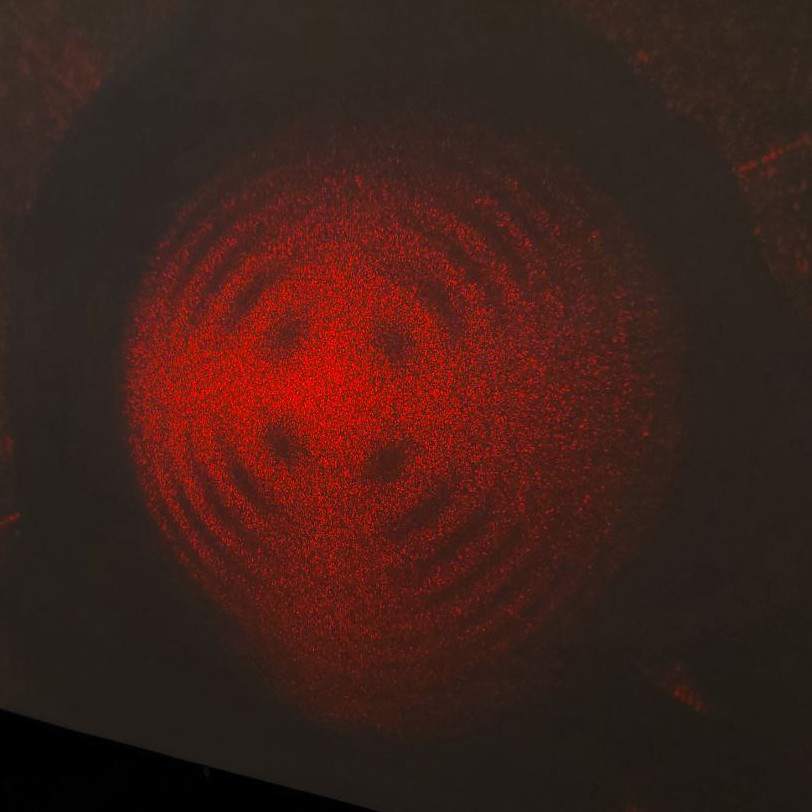
\includegraphics[width=\textwidth]{../Изображения/light.jpg}
		\caption{Разрешённое направление анализатора вертикально.}
	\end{minipage}
\end{figure}

Измерим радиусы тёмных колец $r_m$. \\
\begin{tabular}{|c|c|c|c|c|c|c|}
	\hline
	$N$ & 1 & 2 & 3 & 4 & 5 & 6 \\
	\hline
	$r_m, \mm$ & 27,5 & 39,5 & 49,5 & 56,5 & 63,5 & 70,5 \\
	\hline
\end{tabular}

Построим график зависимости квадрата радиуса тёмного кольца от его порядкового номера $r^2(m)$.

\begin{figure}[H]
	\centering
	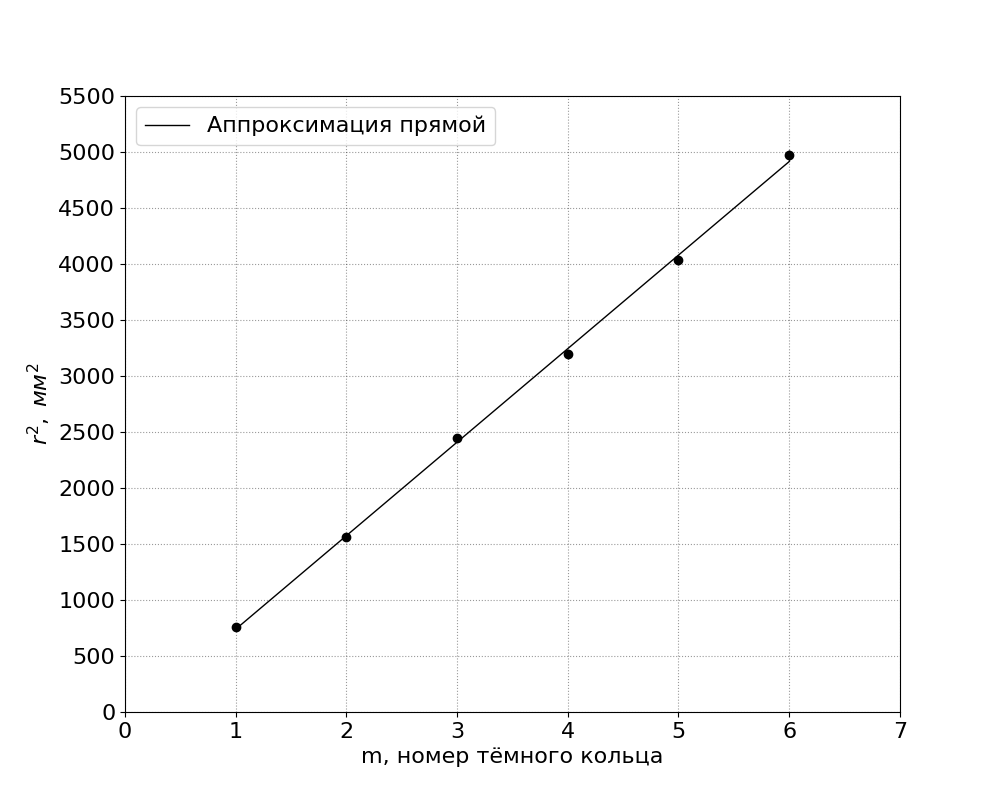
\includegraphics[width=0.6\textwidth]{../Графики/r2(m).png}
	\caption{График зависимости $r^2(m)$}
\end{figure}

Аппроксимируем зависимость прямой $y = a x + b$, по углу наклона определим двулучепреломление $n_o - n_e$. \\
$a = 835 \pm 12 \mm^2$ \\
$b = -95 \pm 47 \mm^2$

$$n_o - n_e = \frac{\lambda}{l}\frac{(n_o L)^2}{a} = 0,097 \pm 0,002$$

Относительную ошибку косвенных измерений оценим по формуле $\varepsilon = \sqrt{4 \cdot \varepsilon_L^2 + \varepsilon_a^2} = 2 \%$.

Определим полуволновое напряжение кристалла ниобата лития. Разрешённое направление анализатора перпендикулярно направлению поляризации лазерного излучения. \\
$U_0 = 0 \V$ (мин). \\
$U_{\frac{\lambda}{2}} = 270 \pm 8 \V$ (макс). \\
$U_{\lambda} = 630 \pm 8 \V$ (мин). \\
$U_{\frac{3\lambda}{2}} = 1020 \pm 8 \V$ (макс). \\
$U_{2\lambda} = 1380 \pm 8 \V$ (мин). \\

Разрешённое направление анализатора параллельно направлению поляризации лазерного излучения. \\
$U_0 = 0 \V$ (макс). \\
$U_{\frac{\lambda}{2}} = 240 \pm 8 \V$ (мин). \\
$U_{\lambda} = 630 \pm 8 \V$ (макс). \\
$U_{\frac{3\lambda}{2}} = 1110 \pm 8 \V$ (мин). \\

Для определения полуволнового напряжения построим графики зависимостей $U(n\frac{\lambda}{2})$. Так как наблюдаемая на экране интенсивность является периодической функцией от напряжения: \\
$I = I_0 \sin^2 \left(\frac{\pi}{2} \frac{U}{U_{\frac{\lambda}{2}}}\right)$ для скрещённых направлений поляроидов \\
$I = I_0 \cos^2 \left(\frac{\pi}{2} \frac{U}{U_{\frac{\lambda}{2}}}\right)$ для параллельных направлений поляроидов.

\begin{figure}[H]
	\centering
	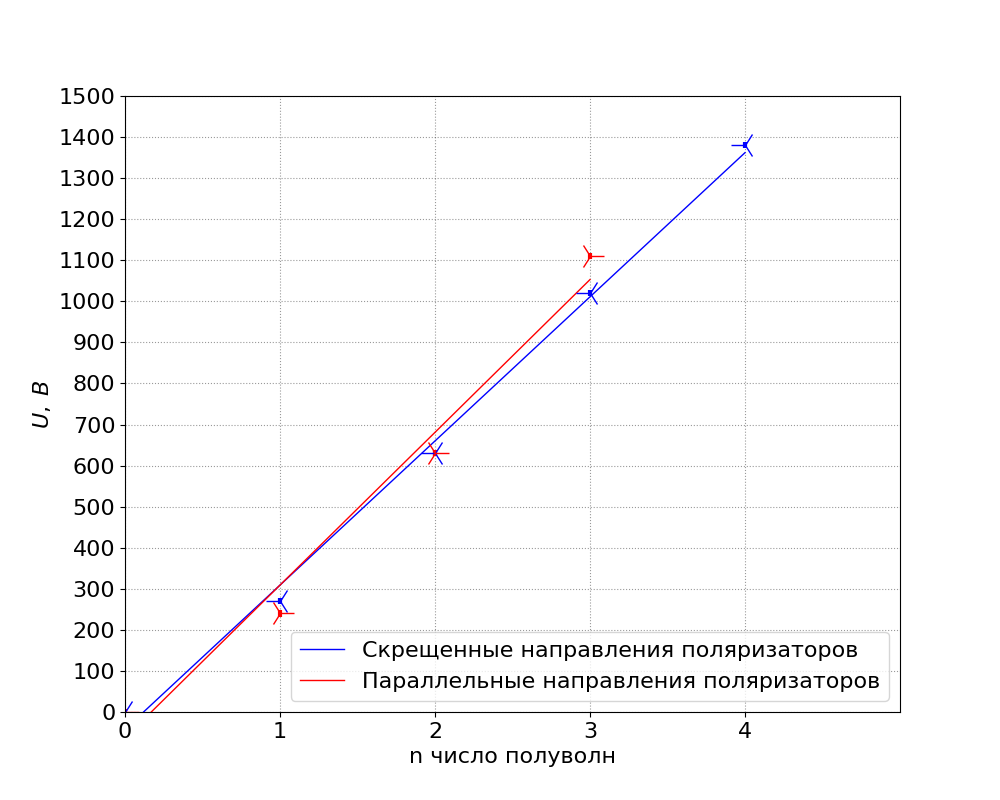
\includegraphics[width=0.6\textwidth]{../Графики/U_lambda.png}
	\caption{График зависимости $U(n\frac{\lambda}{2})$}
\end{figure}

Аппроксимируем зависимости прямыми вида $y = ax + b$: \\
Скрещённые направления поляроидов: \\
$a = 351 \pm 12 \V$ \\
$b = -42 \pm 30 \V$ \\
Параллельных направлений поляроидов: \\
$a = 372 \pm 38 \V$ \\
$b = -63 \pm 71 \V$

За итоговое значение полуволнового напряжения выберем значение $a$ для серии измерений со скрещенными поляроидами, так как в этой серии больше экспериментальных точек. 

Итоговое полуволновое напряжение $U_{\frac{\lambda}{2}} = 351 \pm 12 \V$.

Подадим на кристалл четверть волновое напряжение $U_{\frac{\lambda}{4}} = 150 \pm 8 \V$. Поляризация на выходе кристалла почти круговая, так как при вращении поляроида интенсивность света на экране почти не меняется, хотя небольшие изменения заметны. Варьируя напряжение, было экспериментально установлено, что при данном напряжении изменения интенсивности минимальны.
$U_{\frac{\lambda}{4}}^{рассчётное} = \frac{1}{2} U_{\frac{\lambda}{2}} = 175 \pm 6 \V$.

Заменим экран фотодиодом и подадим на пластинку переменное напряжение. На один вход осциллографа подадим напряжение источника, на другой сигнал с фотодиода. По фигурам Лиссажу определим полуволновое напряжение пластинки. \\
$U_{\frac{\lambda}{2}} = 390 \pm 8 \V$.

Определим коэффициент пропорциональности $A$: $\Delta n = A \cdot E_{эл}$. \\
$A = \frac{\lambda d}{4 U_{\frac{\lambda}{2}} l}$

Для $U = 351 \pm 12 \V$ коэффициент равен $A = (52 \pm 2) \cdot 10^{-12} \; \frac{м}{В}$
\\
Для $U = 390 \pm 8 \V$ коэффициент равен $A = (47 \pm 1) \cdot 10^{-12} \; \frac{м}{В}$